\begin{figure*}
    \centering
        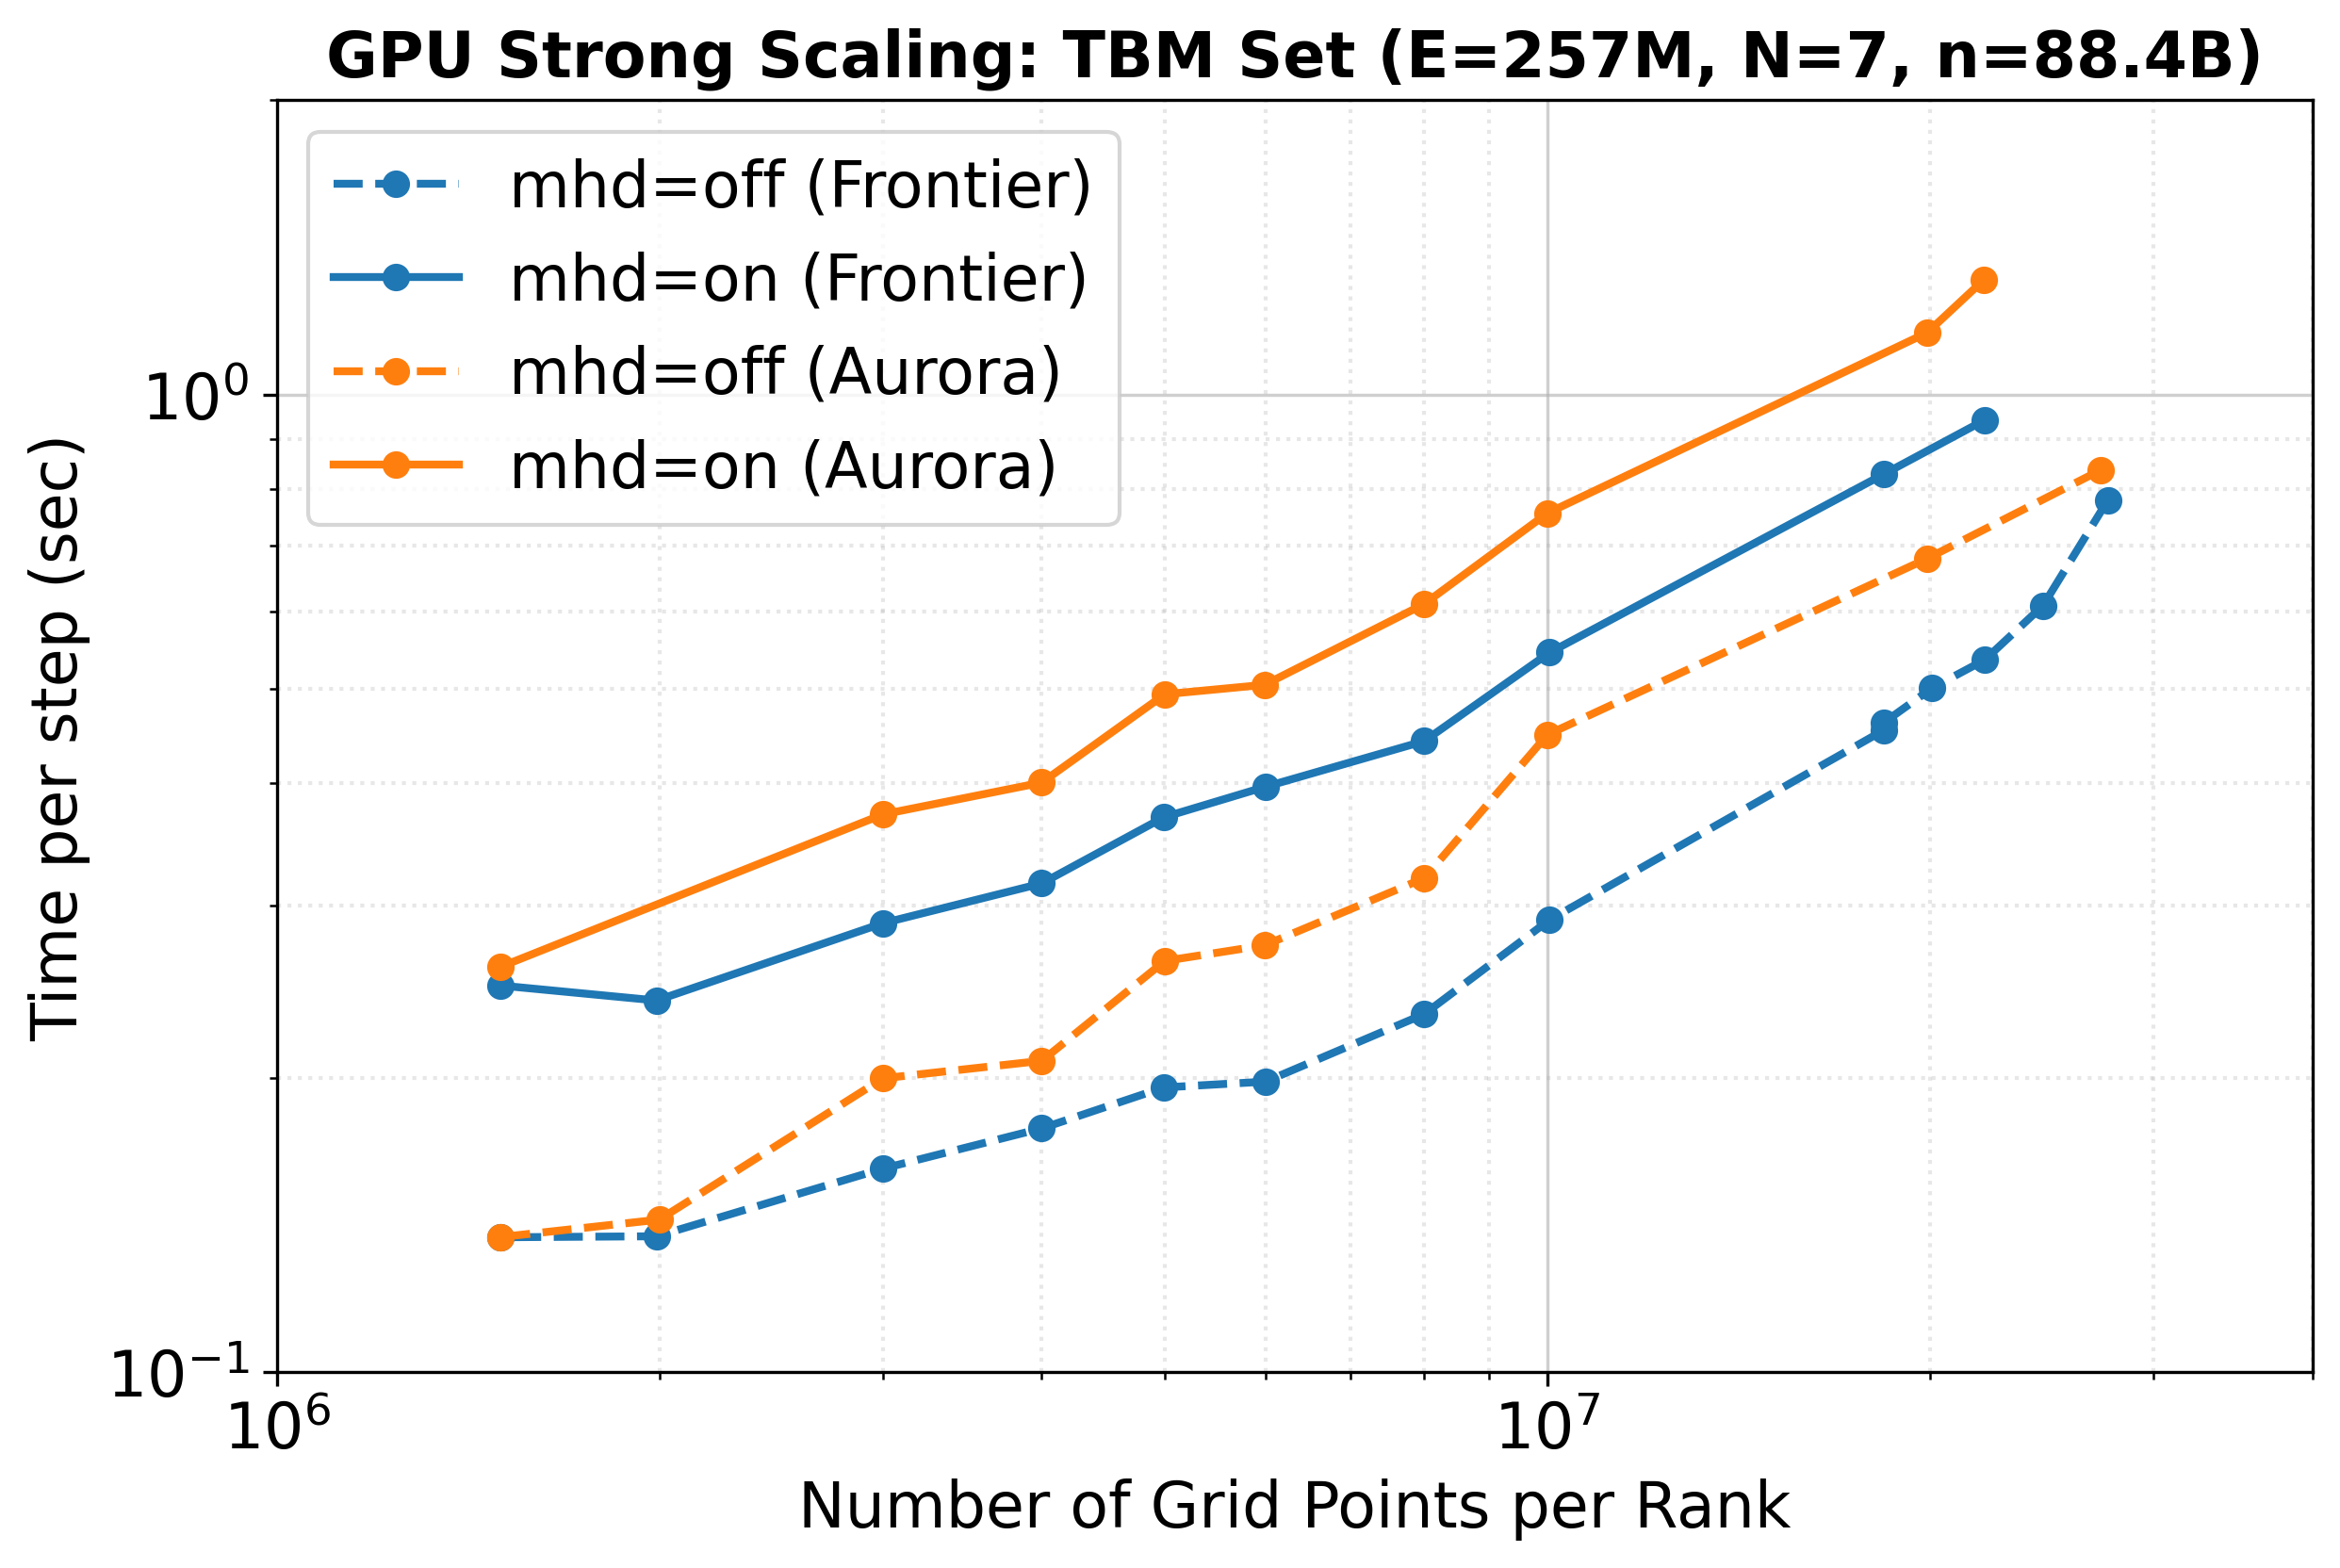
\includegraphics[height=2.1in]{figures/time_per_step_sec_vs_number_of_grid_points_per_rank.png}
        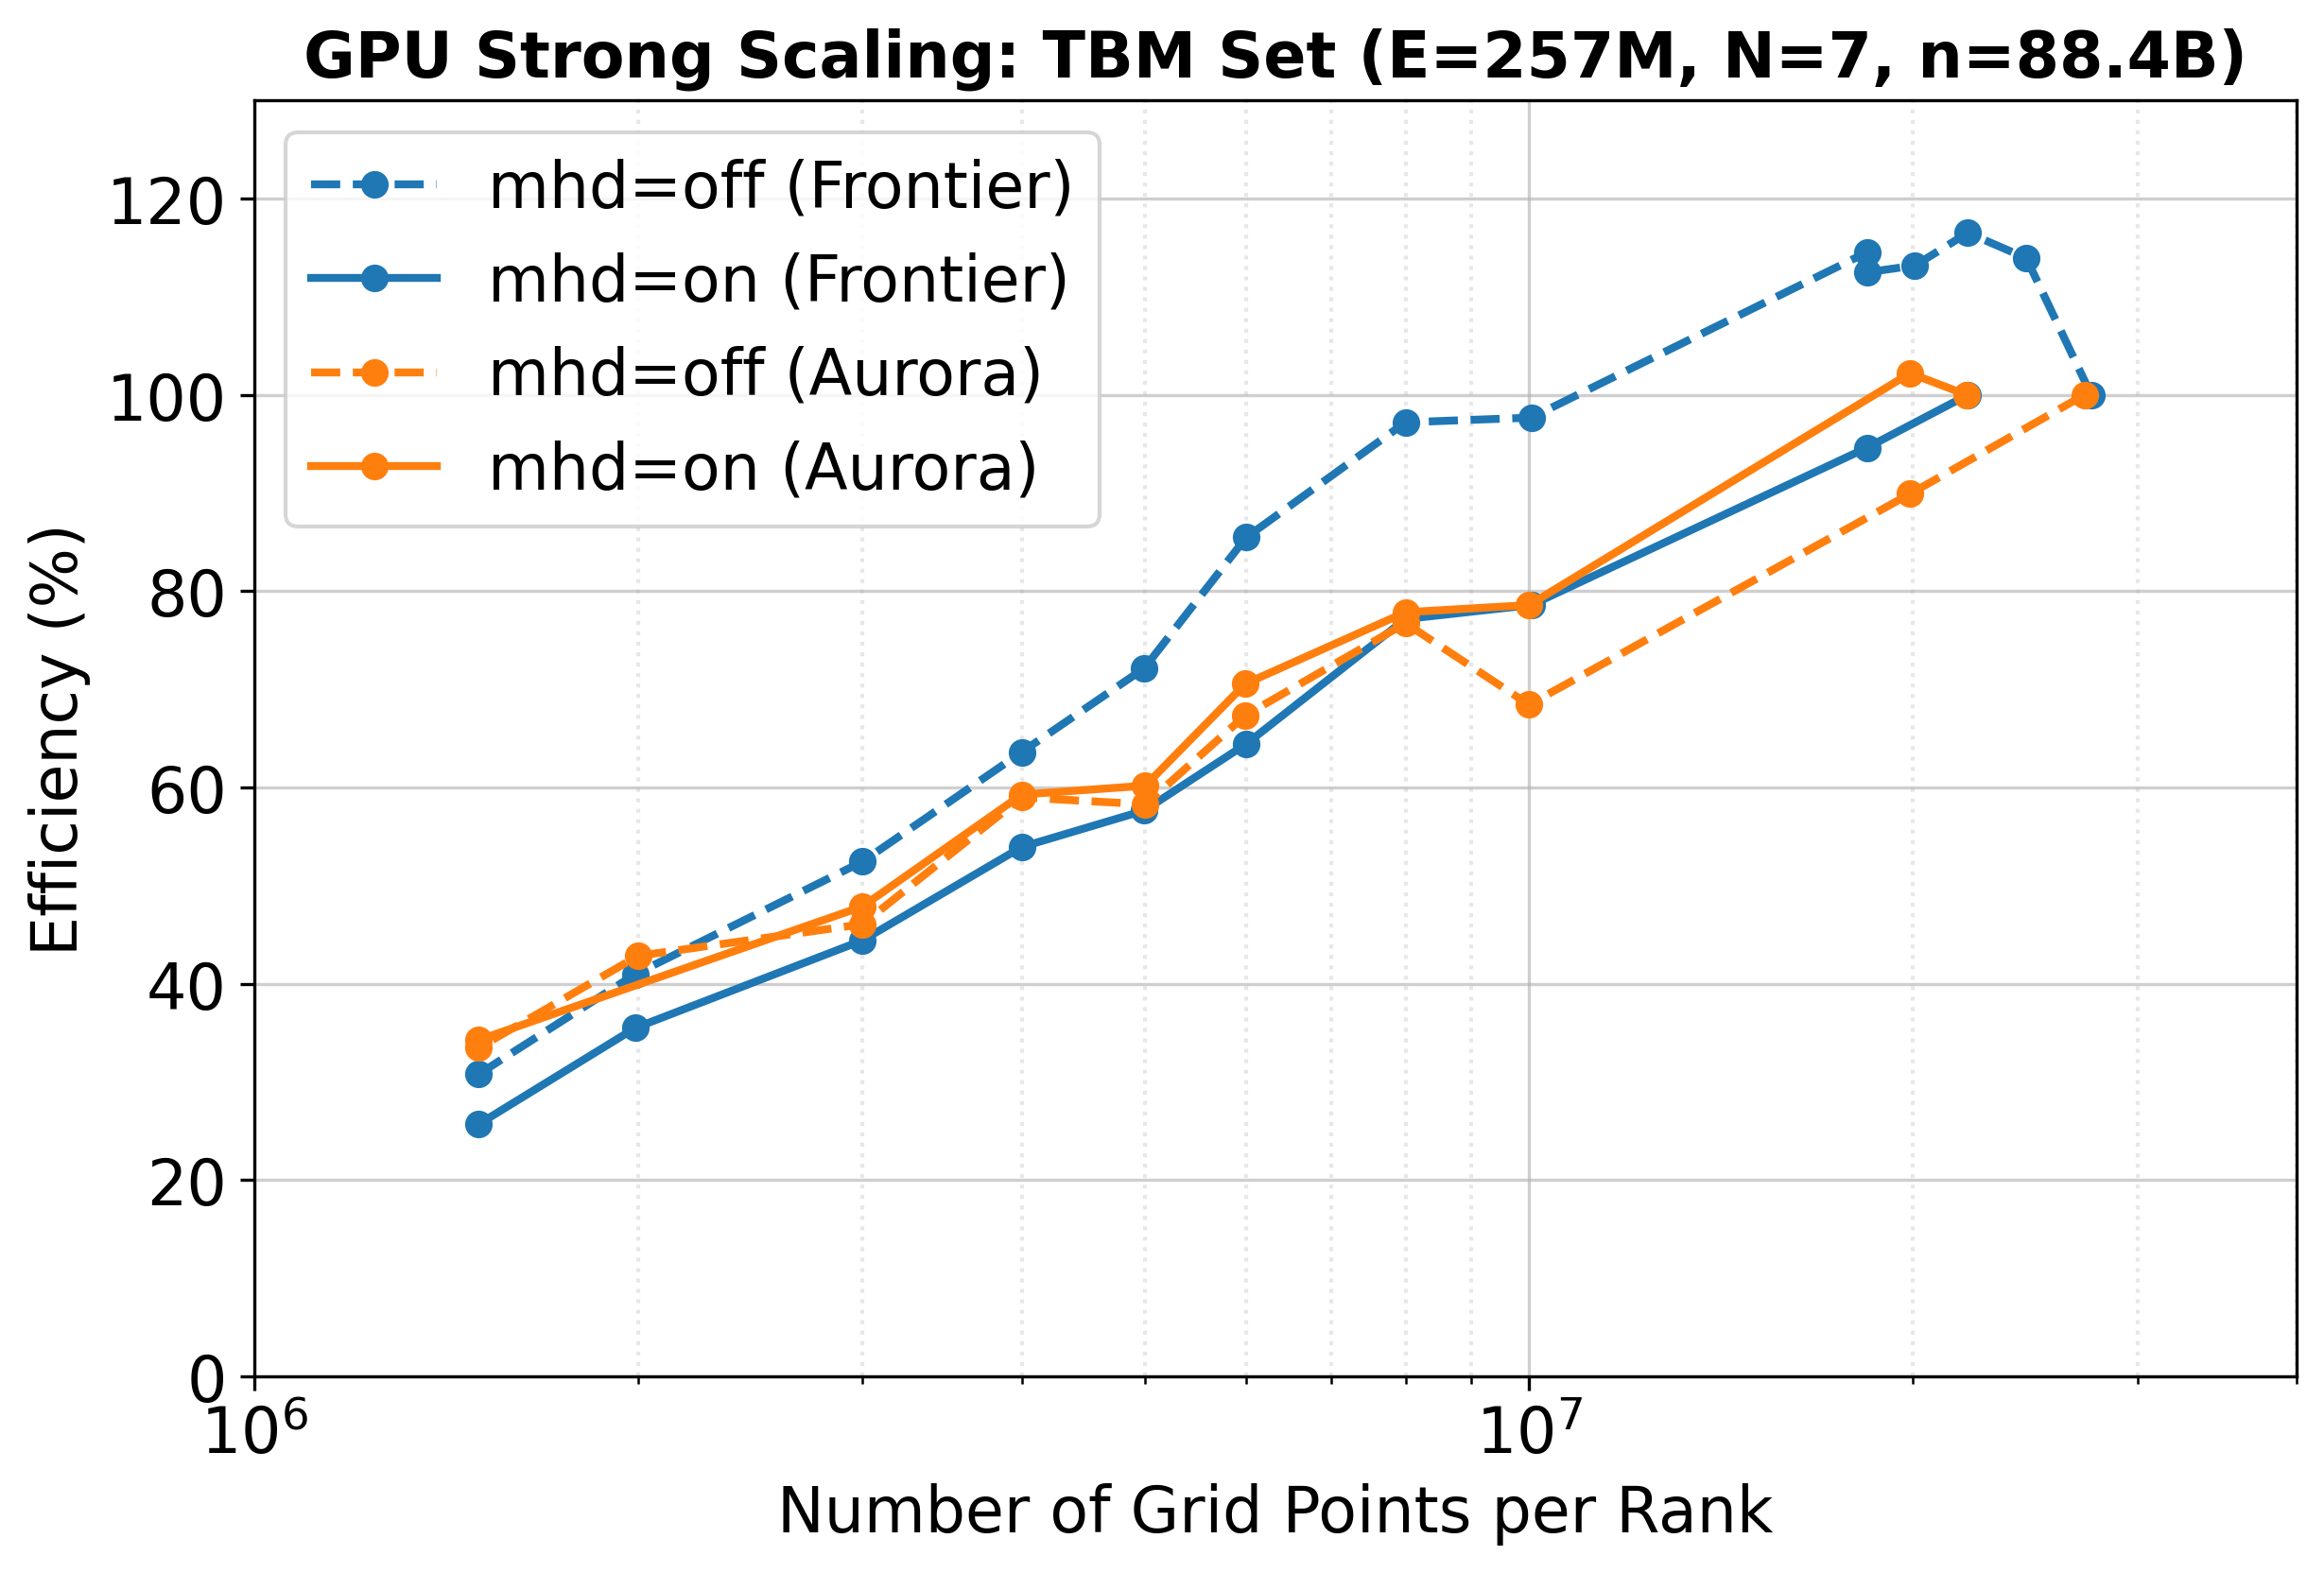
\includegraphics[height=2.1in]{figures/efficiency_vs_number_of_grid_points_per_rank.png}
               \\ \hspace{0.3em}  (a) \hspace{22.5em} (b)  \\
    \caption{\label{fig:v26_strong} Strong scaling tests with and without MHD
    on Frontier and Aurora.}
\end{figure*}

\begin{figure*}
    \centering
        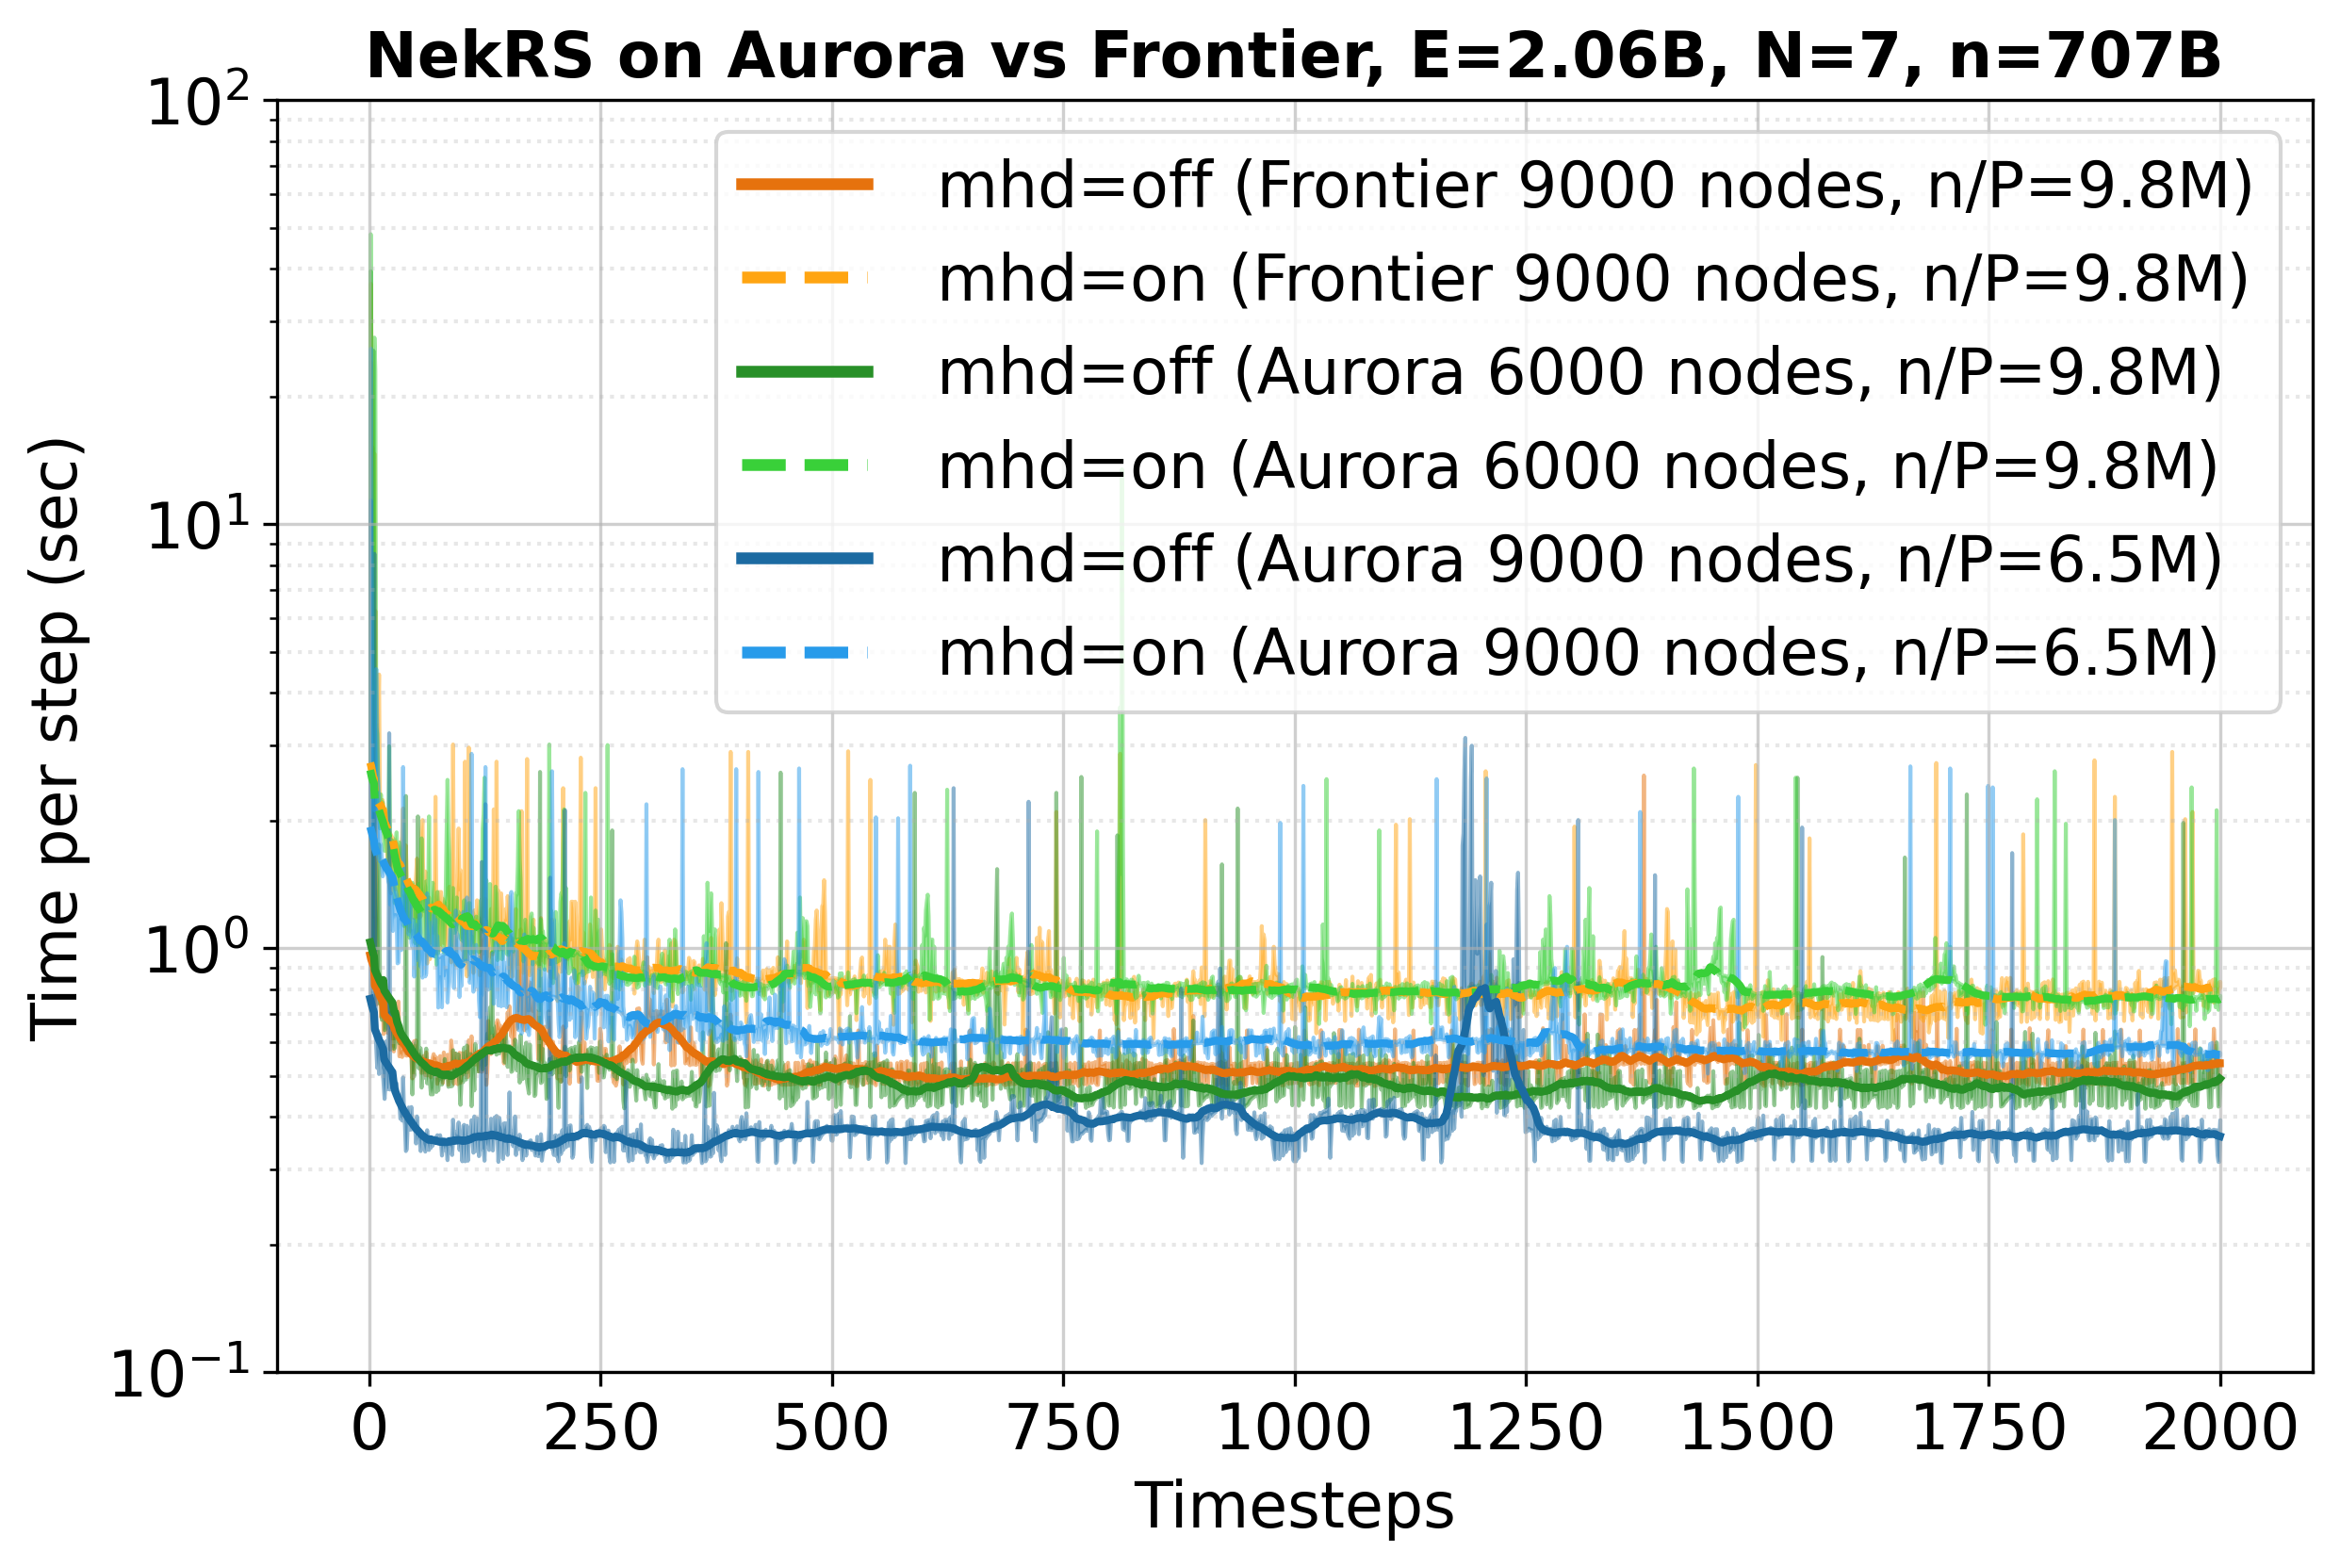
\includegraphics[width=3.1in]{figures/pink_href2_N7.png}
        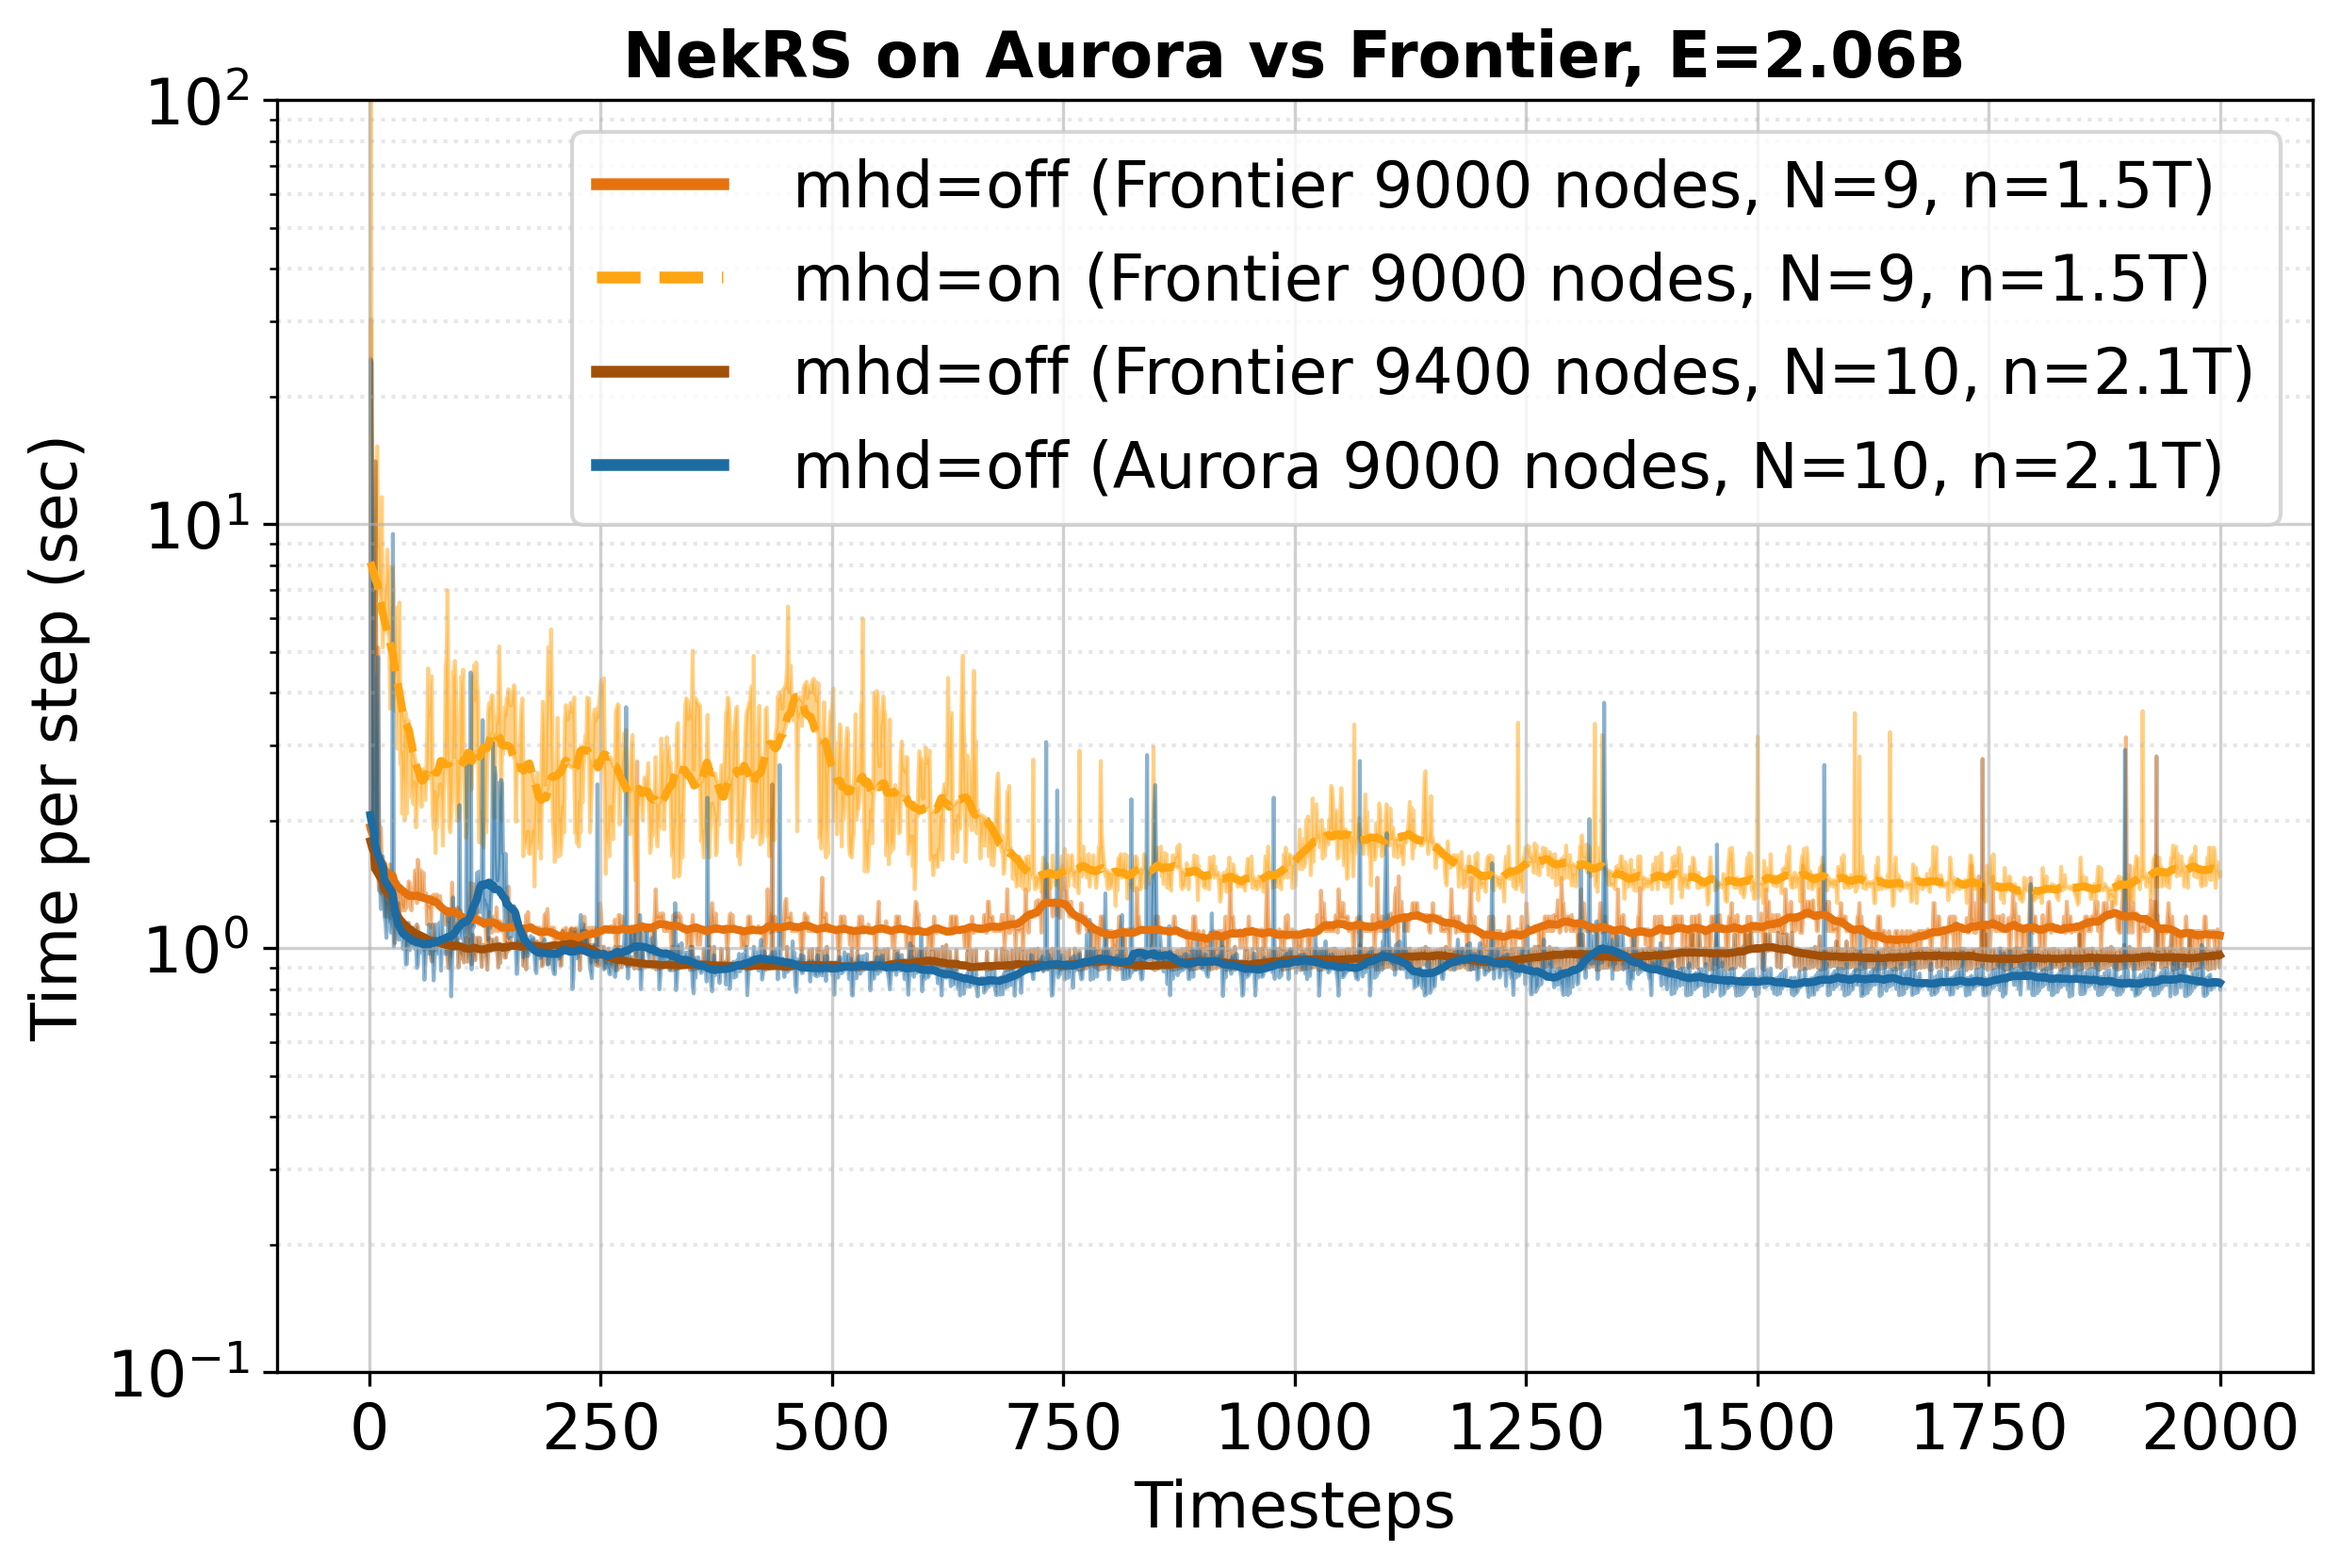
\includegraphics[width=3.1in]{figures/pink_href2_N9_N10.png}
               \\ \hspace{0.3em}  (a) \hspace{22.5em} (b)  \\

    \caption{\label{fig:v26_fullmachine}
    Large-scale NekRS runs on Aurora and Frontier for the TBM set.
    The mesh is $h$-refined to over 2 billion elements, with results shown for
    (a) polynomial order $N=7$ and (b) $N=9$ and $10$, corresponding to
    approximately $1.5$--$2.1$ trillion grid points.}
\end{figure*}


Figure~\ref{fig:v26_strong} shows the strong-scaling behavior on Aurora and
Frontier. Both systems provide 64~GB of memory per GPU tile. Without MHD,
NekRS solves the coupled fluid--thermal system with up to $\sim$27M grid points
per rank, while enabling MHD introduces additional memory overhead and reduces
this limit to $\sim$22M grid points per rank. In the MHD-off configuration, the
solver achieves approximately 80\% parallel efficiency at 5--6M grid points per
rank. With MHD enabled, an additional scalar (electric potential) is solved over
the entire domain, introducing extra coarse-grid solves and reducing the
compute-to-communication ratio. Consequently, the 80\% efficiency threshold
shifts to approximately 8--10M grid points per rank.

Figure~\ref{fig:v26_fullmachine} presents large-scale NekRS runs on Aurora and
Frontier. Frontier (9000 nodes) is already close to full-system scale, whereas
Aurora still offers additional capacity, allowing the node count to increase
from 6000 to 9000. Within the strong-scaling regime, this increase further
reduces time to solution. We push both systems to their limits by increasing the
polynomial order to $N=10$, representing the largest configurations considered.
On Frontier, memory becomes the limiting factor as $N$ increases, and the
$N=10$ case just fits in the MHD-off configuration on 9400 nodes, representing
one of the largest runs to date.




